% Options for packages loaded elsewhere
\PassOptionsToPackage{unicode}{hyperref}
\PassOptionsToPackage{hyphens}{url}
\documentclass[
]{article}
\usepackage{xcolor}
\usepackage[margin=1in]{geometry}
\usepackage{amsmath,amssymb}
\setcounter{secnumdepth}{-\maxdimen} % remove section numbering
\usepackage{iftex}
\ifPDFTeX
  \usepackage[T1]{fontenc}
  \usepackage[utf8]{inputenc}
  \usepackage{textcomp} % provide euro and other symbols
\else % if luatex or xetex
  \usepackage{unicode-math} % this also loads fontspec
  \defaultfontfeatures{Scale=MatchLowercase}
  \defaultfontfeatures[\rmfamily]{Ligatures=TeX,Scale=1}
\fi
\usepackage{lmodern}
\ifPDFTeX\else
  % xetex/luatex font selection
\fi
% Use upquote if available, for straight quotes in verbatim environments
\IfFileExists{upquote.sty}{\usepackage{upquote}}{}
\IfFileExists{microtype.sty}{% use microtype if available
  \usepackage[]{microtype}
  \UseMicrotypeSet[protrusion]{basicmath} % disable protrusion for tt fonts
}{}
\makeatletter
\@ifundefined{KOMAClassName}{% if non-KOMA class
  \IfFileExists{parskip.sty}{%
    \usepackage{parskip}
  }{% else
    \setlength{\parindent}{0pt}
    \setlength{\parskip}{6pt plus 2pt minus 1pt}}
}{% if KOMA class
  \KOMAoptions{parskip=half}}
\makeatother
\usepackage{graphicx}
\makeatletter
\newsavebox\pandoc@box
\newcommand*\pandocbounded[1]{% scales image to fit in text height/width
  \sbox\pandoc@box{#1}%
  \Gscale@div\@tempa{\textheight}{\dimexpr\ht\pandoc@box+\dp\pandoc@box\relax}%
  \Gscale@div\@tempb{\linewidth}{\wd\pandoc@box}%
  \ifdim\@tempb\p@<\@tempa\p@\let\@tempa\@tempb\fi% select the smaller of both
  \ifdim\@tempa\p@<\p@\scalebox{\@tempa}{\usebox\pandoc@box}%
  \else\usebox{\pandoc@box}%
  \fi%
}
% Set default figure placement to htbp
\def\fps@figure{htbp}
\makeatother
\setlength{\emergencystretch}{3em} % prevent overfull lines
\providecommand{\tightlist}{%
  \setlength{\itemsep}{0pt}\setlength{\parskip}{0pt}}
\usepackage{graphicx}
\usepackage{float}
\usepackage{tikz}
\usepackage{xcolor}
\usepackage{amsmath}
\usepackage{bookmark}
\IfFileExists{xurl.sty}{\usepackage{xurl}}{} % add URL line breaks if available
\urlstyle{same}
\hypersetup{
  hidelinks,
  pdfcreator={LaTeX via pandoc}}

\author{}
\date{\vspace{-2.5em}}

\begin{document}

\section{Question}\label{question}

Un arquitecto tiene un cilindro de forma cilíndrica. El cilindro tiene
una base circular de radio 2 cm y una altura de 10 cm, como se muestra
en la figura.

\begin{center}
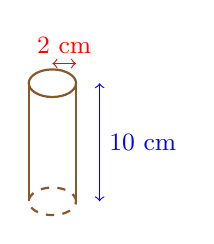
\begin{tikzpicture}[scale=0.5]
% Definir parámetros del cilindro
\def\radio{0.6}
\def\altura{3}
\def\profundidad{0.35}

% Elipse superior (tapa visible)
\draw[thick, brown!70!black] (0, \altura) ellipse (\radio cm and \profundidad cm);

% Elipse inferior (base) - solo la parte visible (atrás)
\draw[thick, brown!70!black, dashed] (0, 0) ellipse (\radio cm and \profundidad cm);

% Líneas laterales del cilindro
\draw[thick, brown!70!black] (-\radio, 0) -- (-\radio, \altura);
\draw[thick, brown!70!black] (\radio, 0) -- (\radio, \altura);

% Etiqueta del radio - elevada para evitar solapamiento con la tapa
\draw[<->, red] (0, \altura + 0.5) -- (\radio, \altura + 0.5) node[midway, above, font=\small, transform shape=false] {2 cm};

% Etiqueta de la altura
\draw[<->, blue] (\radio + 0.6, 0) -- (\radio + 0.6, \altura) node[midway, right, font=\small, transform shape=false] {10 cm};

\end{tikzpicture}
\end{center}

A partir de la información anterior, el arquitecto plantea la siguiente
operación:

\[\pi \times 2^2 \times 10 = 125.66\]

\textbf{¿A qué corresponde el resultado de la anterior operación?}

\subsection{Answerlist}\label{answerlist}

\begin{itemize}
\tightlist
\item
  Al perímetro de la tapa del cilindro.
\item
  Al área de la tapa del cilindro.
\item
  Al volumen del cilindro.
\item
  Al área lateral del cilindro.
\end{itemize}

\section{Solution}\label{solution}

Para resolver este problema, debemos identificar qué magnitud geométrica
corresponde a la expresión matemática planteada.

\subsubsection{Análisis de la
operación}\label{anuxe1lisis-de-la-operaciuxf3n}

La operación planteada es:

\[\pi \times 2^2 \times 10 = 125.66\]

Donde:

\begin{itemize}
\tightlist
\item
  \(r = 2\) cm (radio de la base circular)
\item
  \(h = 10\) cm (altura del cilindro)
\end{itemize}

\subsubsection{Fórmulas relevantes del
cilindro}\label{fuxf3rmulas-relevantes-del-cilindro}

Para un cilindro de radio \(r\) y altura \(h\), tenemos las siguientes
fórmulas:

\begin{enumerate}
\def\labelenumi{\arabic{enumi}.}
\tightlist
\item
  \textbf{Volumen del cilindro:} \(V = \pi r^2 h\)
\item
  \textbf{Área de la tapa (círculo):} \(A_{tapa} = \pi r^2\)
\item
  \textbf{Perímetro de la tapa (circunferencia):} \(P_{tapa} = 2\pi r\)
\item
  \textbf{Área lateral del cilindro:} \(A_{lateral} = 2\pi r h\)
\end{enumerate}

\subsubsection{Comparación con la operación
dada}\label{comparaciuxf3n-con-la-operaciuxf3n-dada}

La expresión \(\pi \times 2^2 \times 10\) tiene la estructura:

\[\pi \times r^2 \times h\]

Comparando con las fórmulas anteriores, observamos que \textbf{esta
expresión corresponde exactamente a la fórmula del volumen del
cilindro}:

\[V = \pi r^2 h = \pi \times 2^2 \times 10 = 125.66 \text{ cm}^3\]

\subsubsection{Verificación de otras
opciones}\label{verificaciuxf3n-de-otras-opciones}

Verifiquemos por qué las otras opciones son incorrectas:

\textbf{Área de la tapa:}
\[A_{tapa} = \pi r^2 = \pi \times  2 ^2 =  12.57  \text{ cm}^2\] Esta
fórmula NO incluye la altura.

\textbf{Perímetro de la tapa:}
\[P_{tapa} = 2\pi r = 2 \times \pi \times  2  =  12.57  \text{ cm}\]
Esta fórmula NO incluye \(r^2\) ni la altura.

\textbf{Área lateral:}
\[A_{lateral} = 2\pi r h = 2 \times \pi \times  2  \times  10  =  125.66  \text{ cm}^2\]
Esta fórmula NO incluye \(r^2\) (solo \(r\)).

\subsubsection{Conclusión}\label{conclusiuxf3n}

La operación \(\pi \times 2^2 \times 10 = 125.66\) corresponde al
\textbf{volumen del cilindro}, medido en centímetros cúbicos (cm³).

La estructura \(\pi r^2 h\) es característica de la fórmula del volumen
de un cilindro, donde:

\begin{itemize}
\tightlist
\item
  \(\pi r^2\) representa el área de la base circular
\item
  Al multiplicar por la altura \(h\), obtenemos el volumen total
\end{itemize}

\subsection{Answerlist}\label{answerlist-1}

\begin{itemize}
\tightlist
\item
  Falso. El perímetro de la tapa sería \(2\pi r\) (no incluye \(r^2\) ni
  altura).
\item
  Falso. El área de la tapa sería \(\pi r^2\) (sin la altura).
\item
  Verdadero. La fórmula \(\pi r^2 h\) corresponde al volumen del
  cilindro.
\item
  Falso. El área lateral sería \(2\pi r h\) (con \(r\) en lugar de
  \(r^2\)).
\end{itemize}

\section{Meta-information}\label{meta-information}

exname: volumen\_cilindro\_interpretacion\_formula extype: schoice
exsolution: 0010 exshuffle: TRUE exsection:
Geometría\textbar Cilindro\textbar Volumen\textbar Interpretación
exextra{[}Type{]}: Interpretación y representación exextra{[}Level{]}: 2
exextra{[}Language{]}: es exextra{[}Course{]}: Matemáticas ICFES
exextra{[}Componente{]}: Geométrico-Métrico exextra{[}Pensamiento{]}:
Métrico y Espacial

\end{document}
